%----------------------------------------------------------------------------------------
%	Inställningar och dokumentkonfiguration
%----------------------------------------------------------------------------------------

\documentclass[paper=a4, fontsize=11pt]{report} % A4-sida och 11 punkters fontstorlek

\usepackage[T1]{fontenc} % 8-bitarskodning som har 256 glyfer
\usepackage[swedish]{babel} % Svenskt språk
\usepackage[utf8]{inputenc} % För svenska tecken
\usepackage{dtk-logos} % Logos
\usepackage{wallpaper} % Bakgrundsbild
\usepackage{fancyhdr} % Specialsidhuvud och sidfot
\usepackage{enumerate} 
\usepackage{xifthen}% provides \isempty test
\usepackage{listings}% Code examples
\usepackage{xcolor}

\lstdefinestyle{BashInputStyle}{
  language=bash,
  basicstyle=\small\sffamily,
  numbers=left,
  numberstyle=\tiny,
  numbersep=3pt,
  frame=tb,
  columns=fullflexible,
  backgroundcolor=\color{yellow!20},
  linewidth=0.9\linewidth,
  xleftmargin=0.1\linewidth
}
% Exampels
% Inline
% \lstinline[style=BashInputStyle]´# apt-get --purge remove rubygems´.
% Multiline
% \begin{lstlisting}[style=BashInputStyle]
%    # apt-get --purge remove rubygems
% \end{lstlisting}

\pagestyle{fancyplain} % Använd sidhuvud och sidfot på alla sidor
\fancyhead[L]{Seminar 1 -- 1DV720 -- \the\year -- Server Administration} % Titel till vänster i sidhuvud
\fancyhead[C]{} % Tomt i mitten
\fancyhead[R]{} % Tomt till höger
\fancyfoot[L]{} % Tomt till vänster
\fancyfoot[C]{} % Tomt i mitten
\fancyfoot[R]{\thepage} % Sidnumrering till höger i sidfoten
\renewcommand\thesection{\arabic{section}} % Section beter sig som i dokumentklassen article

\newcommand{\win}[1]{Microsoft Windows Server\ifthenelse{\isempty{#1}}{}{ #1}}
\newcommand{\gui}[0]{``Server with a GUI''}
\newcommand{\core}[0]{Windows Server Core}
%----------------------------------------------------------------------------------------
%	TITLE SECTION
%----------------------------------------------------------------------------------------
\newcommand\BackgroundPic{
    \put(-50,-50){
    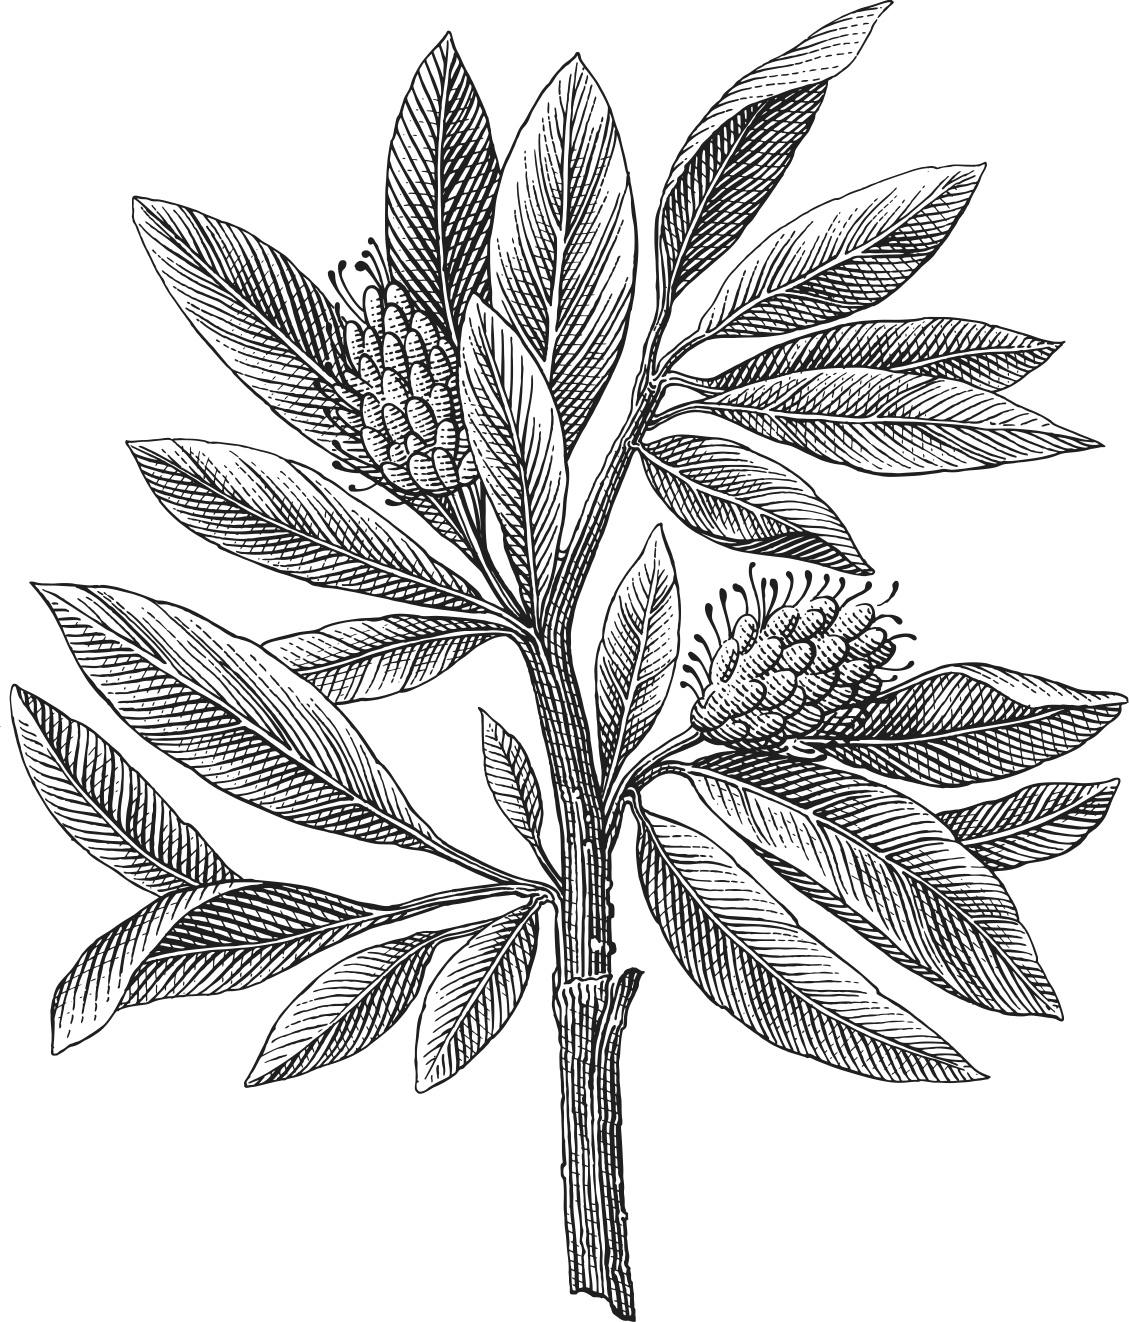
\includegraphics[keepaspectratio,scale=0.65]{lnu_etch.png} % Bakgrundsbild
    }
}
\newcommand\BackgroundPicLogo{
    \put(15,700){
    
\includegraphics[keepaspectratio,scale=0.10]{logo.png} % Logga i vänstra hörnet
    }
}

\newcommand{\horrule}[1]{\rule{\linewidth}{#1}} % Skapa hortisontell linje

\title{	\vspace{-10cm}
    \normalfont \normalsize
    \textsc{Linnaeus University} \\ [25pt] % Universitetes namn
    \horrule{0.5pt} \\[0.4cm] % Tunn linje högst upp
    \huge Seminar 1\\ % Arbetes titel
	\large \textcolor{gray}{1DV720 -- Server Administration}
    \horrule{0.5pt} \\[0.4cm] % Tunn linje längst ner
}

\author{Jacob Lindehoff} % Författarnas namn

\date{\normalsize\today} % Dagens datum

\begin{document}
\AddToShipoutPicture*{\BackgroundPic} % Lägger in backgrundsbild på första sidan
\AddToShipoutPicture*{\BackgroundPicLogo}
\maketitle % Skriv ut titeln
\noindent % Tabba inte in på första meningen

%------------------------------------------------
%	Introduktion
%------------------------------------------------
\section{Introduction}
During this seminar, we will address the following topics:
\begin{itemize}
\item Server vs. Client
\item Installation of various server operating systems
\item Basic configuration
\item Administrative Tools

\end{itemize}

%------------------------------------------------
%	Deadline
%------------------------------------------------
\section{Deadline}
The seminar is on the {\color{red}23th January 2018} and it is compulsory. If you cannot participate, it must be notified in advance and a written report of the seminar must be submitted no later than {\color{red}3 days} after the seminar. The written report should contain detailed answers to all questions in the seminar.
\newpage
%------------------------------------------------
%	Seminariefrågor
%------------------------------------------------
\section{Seminar Questions}

\begin{enumerate}
    \begin{large}
    \subsection{General}
        \item What is it that makes a computer to a server (hardware)?
        \item What is meant by a Server when talking about software?
        \item What are the major historical milestones for:
            \begin{enumerate}[a.]
                \item \win{}
                \item Linux
            \end{enumerate}
        \item Describe the different types of System administrator roles and which you are most interested in working as?
        \item You have a client who has 50 clients, they want a new file server.
            \begin{enumerate}[a.]
                \item How do you find appropriate hardware for the company?
                \item What hardware do you recommend?
            \end{enumerate}
        \item What is important to consider before installing a server operating system?
        \item What is a HCL and why should it be checked before you install server operating system?
        \subsection{Microsoft Windows Server}
        \item Client Access Licenses
            \begin{enumerate}[a.]
                \item What are the different CALs that Microsoft has?
                \item How do the different CALs work?
                \item How would you do to choose the right CAL, in which scenarios does the different CALs fit?
            \end{enumerate}
        \item \core
            \begin{enumerate}[a.]
                \item What is \core?
                \item In which scenarios is a Server Core installation appropriate?
                \item What advantages does a \core{} installation compared with a \gui?
            \end{enumerate}
        \item Windows Powershell and Windows Command Prompt
            \begin{enumerate}[a.]
                \item What is Windows Powershell?
                \item What is the difference between Windows Command Prompt and Powershell?
                \item Name and explain 10 useful command prompt tools/commands.
                \item Name and explain 10 useful Powershell cmdLets.
            \end{enumerate}
        \item How does Windows Advanced Firewall work?
        
        \noindent \subsection{Linux}
        \item There are a lot of different Linux distributions, choose three of the major distributions and answer the following questions:
            \begin{enumerate}[a.]
                \item What are the 5 biggest differences between the distributions?
                \item What did you choose these distributions?
            \end{enumerate}
        \item What should you consider when you are choosing a Linux distribution for a project?
       
       
%------------------------------------------------
%	Grundläggande
%------------------------------------------------       
        \item What does the following Bash programs do, explain 2-3 [options] on each and how to use them:
            \begin{enumerate}[a.]
	
		\item man
		\item echo
		\item sudo
		\item cat
		\item ls
		\item mv
		\item cp
		\item alias

            \end{enumerate}

	\item Look into how to handle a text editor such as nano(recommended), vim or emacs. You should be able to edit/create files and search for patterns.
	
	\item How can you search for - and install software on your distribution?
	
	\item Locate the log files of your Linux distribution does it have a specific folder that stores it or does it use a command such as journalctl?

	\item What is a pipe? '|'
	
%------------------------------------------------
%	S IPtables
%------------------------------------------------        
        \item IPTables
            \begin{enumerate}[a.]
                \item What is IPTables?
                \item How do you manage IPTables?
                \item Name some basic IPTables commands?
                \item What does the following two lines do together and separate. What would be the difference if we had ACCEPT instead of DROP using both settings?
                \newline
                \lstinline[style=BashInputStyle]"sudo iptables --policy INPUT DROP"
		\newline
                \lstinline[style=BashInputStyle]"sudo iptables -A INPUT -m conntrack --ctstate ESTABLISHED,RELATED -j ACCEPT" 
		\newline
		\item What is the difference between inserting(\lstinline[style=BashInputStyle]'iptables -A [...]') a rule and appending it? Does it matter where the rule is put?
		
            \end{enumerate}
       
    \end{large}
\end{enumerate}
\end{document}
